\documentclass[11pt,a4paper]{article}

\usepackage[margin=2.1cm,top=2.3cm,bottom=2.3cm]{geometry}
\usepackage{amsmath,amssymb}
\usepackage{mathtools}
\usepackage[T1]{fontenc}
\usepackage{lmodern}
\usepackage{microtype}
\usepackage{xcolor}
\usepackage{enumitem}
\usepackage{fancyhdr}
\usepackage[most]{tcolorbox}
\usepackage{tikz}
\usetikzlibrary{arrows.meta,decorations.pathreplacing,patterns}
\usepackage[hidelinks]{hyperref}

\definecolor{ink}{RGB}{25,25,25}
\definecolor{boxline}{RGB}{70,70,70}

\newtcolorbox{handbox}{
  enhanced,
  colback=white,
  colframe=boxline,
  boxrule=0.8pt,
  arc=1.2mm,
  left=5pt, right=5pt, top=4pt, bottom=4pt,
  before skip=7pt, after skip=7pt
}

\newtcolorbox{notebox}[1][]{
  enhanced,
  colback=black!3,
  colframe=black!35,
  boxrule=0.6pt,
  arc=0.8mm,
  left=6pt, right=6pt, top=4pt, bottom=4pt,
  fonttitle=\bfseries\small,
  title={#1}
}

\pagestyle{fancy}
\fancyhf{}
\fancyhead[L]{\small Phy 324 --- Numerical Methods}
\fancyhead[R]{\small Transcription of \texttt{01.pdf}}
\fancyfoot[C]{\small\thepage}
\renewcommand{\headrulewidth}{0.4pt}

\setlength{\parindent}{0pt}
\setlength{\parskip}{5pt}
\setlist[itemize]{leftmargin=1.4em,itemsep=1pt,topsep=2pt}
\setlist[enumerate]{leftmargin=1.7em,itemsep=1pt,topsep=2pt}

\newcommand{\pagehead}[1]{%
  \clearpage
  \section*{Page #1}
  \vspace{-0.6em}
  {\color{black!45}\rule{\linewidth}{0.5pt}}
  \vspace{0.4em}
}
\newcommand{\ann}[1]{{\small\itshape #1}}
\newcommand{\circled}[1]{\textcircled{\scriptsize #1}}

\title{\vspace{-1.5cm}\textbf{Phy 324 --- Numerical Methods}\\[4pt]
\large Transcription of the handwritten notes in \texttt{01.pdf}}
\author{}
\date{}

\begin{document}
\maketitle
\vspace{-0.8cm}

\begin{notebox}[About this transcription]
This document reproduces, page by page, the handwritten notes contained in
\texttt{01.pdf} (29 pages; the last page is blank). All headings, formulas,
boxed results, annotations and diagrams have been transcribed. The sketches
have been redrawn with TikZ. Handwriting that is ambiguous is reproduced as
read; original spellings and abbreviations (e.g.\ ``soln'', ``eqn'',
``poly.'') are retained.
\end{notebox}

%============================================================
\pagehead{1}

\textbf{\underline{Phy 324:}}

Merge 2 lecture into 1 and make it to a tutorial session

Possible marks distribution
\[
\begin{array}{rcl}
20 \to \text{Internal} & \longrightarrow & 10\ \text{marks (Attendance + Assignment)}\\[2pt]
                       & \longrightarrow & 10\ \text{marks (Tutorial \& Quiz)}\\[6pt]
30 \to \text{Midsem}\\[2pt]
50 \to \text{Endsem}
\end{array}
\]

Numerical Analysis --- Timings dates

\subsection*{Root finding Methods}

\textbf{\underline{Bisection Method}}

\begin{center}
\begin{tikzpicture}[scale=1.0,>=Stealth]
  \draw[->] (-0.2,0) -- (6.4,0) node[right] {$x$};
  \draw[->] (0.3,-2.4) -- (0.3,2.8);
  \draw[thick] (0.8,2.1) .. controls (1.5,2.0) and (1.7,0.25) .. (2.55,0.1)
               .. controls (3.25,0.0) and (3.35,-1.7) .. (4.15,-1.45);
  \fill (1.25,0) circle (1.6pt) node[below=3pt] {$a$};
  \fill (2.55,0) circle (1.6pt) node[below=3pt] {$c$};
  \fill (4.15,0) circle (1.6pt) node[below=3pt] {$b$};
  \draw[dashed] (2.55,0) -- (2.55,0.9);
  \draw[dashed] (4.15,0) -- (4.15,-0.75);
  \node[above right] at (3.02,0.28) {\small root};
  \draw[<->] (1.25,-1.85) -- (4.15,-1.85) node[midway,below] {1st interval};
  \draw[<->] (1.25,2.40) -- (2.55,2.40) node[midway,above] {2nd interval};
\end{tikzpicture}
\end{center}

\begin{verbatim}
while (b-a)/2 > TOL:
    c = (a+b)/2
    if f(c) = 0 , stop end
    if f(a)f(c) <= 0
        b = c
    else
        a = c
    end
end
Answer root => (a+b)/2
\end{verbatim}

\textbf{\underline{Newton--Raphson Method:}}

Take an initial guess $x_0$
\[
f(x)=f(x_0)+(x-x_0)f'(x_0)=0
\]
\begin{handbox}
\[
\Rightarrow\quad \boxed{\,x=x_0-\frac{f(x_0)}{f'(x_0)}\,}
\]
\end{handbox}

%============================================================
\pagehead{2}

\textbf{\underline{Bisection Error}}

\[
\begin{rcases}
e_0=(b-a)\\
e_1=\dfrac{b-a}{2}\\
\vdots\\
e_n=\dfrac{b-a}{2^n}
\end{rcases}
\;\Rightarrow\; e_{n+1}=\frac{e_n}{2}
\qquad\text{(Order of linear)}
\]

$r=$ root of $f(x)$ $\Rightarrow f(r)=0$

$x_0=$ initial guess
\[
f(r)=f(x_0)+(r-x_0)f'(x_0)+\frac{(r-x_0)^2}{2!}f''(x_0)
\]
\[
0=\frac{f(x_0)}{f'(x_0)}+(r-x_0)+\frac{(r-x_0)^2}{2!}\frac{f''(x_0)}{f'(x_0)}
\]
\[
\Rightarrow\; -\frac{f(x_0)}{f'(x_0)}=(r-x_0)+\frac{(r-x_0)^2}{2!}\frac{f''(x_0)}{f'(x_0)}
\]
\[
\Rightarrow\; x_i-\frac{f(x_i)}{f'(x_i)}-r=\frac{(r-x_i)^2}{2!}\frac{f''(x_i)}{f'(x_i)}
\]
\begin{handbox}
\[
\Rightarrow\quad x_{i+1}-r=\frac{(r-x_i)^2}{2}\,\frac{f''(x_i)}{f'(x_i)}
\]
\end{handbox}
\begin{handbox}
\[
\Rightarrow\quad e_{i+1}=\frac{e_i^2}{2}\,\frac{f''(x_i)}{f'(x_i)}
\]
\end{handbox}
\begin{handbox}
\[
\text{Let}\qquad \frac{e_{i+1}}{e_i^2}=\frac12\,\frac{f''(r)}{f'(r)}
\]
\end{handbox}
\[
e_{i+1}\propto e_i^2
\]
Error at $i$th iteration $=e_i$

%============================================================
\pagehead{3}

\textbf{\underline{Linear convergence of Newton Raphson}}

\[
x_{i+1}=x_i-\frac{f(x_i)}{f'(x_i)}
\qquad\qquad \text{Let } f(x)=x^2
\]
\[
x_{i+1}=x_i-\frac{x_i^2}{2x_i}=\frac{x_i}{2}
\]

Error at $i$th iteration $=x_i-r$

Since there is linear convergence of error $\Rightarrow$ Newton Raphson is
linear but is linearly convergent, because $x^2$ doesn't cut through the
$x$-axis linearly.

Limited $\Rightarrow$ this happen because $x^2$ doesn't cut through the
$x$-axis linearly.

\subsection*{Multiplicity of root:}

Given $f(x)$ we can write
\[
f(x)=(x-r)^m g(x)
\]
where $r$ is a root of $f(x)$. Here $m\to$ multiplicity of root.

\textbf{Note:} given a $f(x)$ has root $r$ with multiplicity ``$m$''
\[
f(r)=0,\ \dots,\ f^{(m-1)}(r)=0 \quad\&\quad f^{(m)}(r)\neq 0
\]
This is the way to get the multiplicity of $f$.

\begin{handbox}
``If root $r$ has multiplicity is 1, then error convergence is quadratic.''
\end{handbox}
$\hookrightarrow$ Check this!!!

%============================================================
\pagehead{4}

To prove quadratic convergence, we use \textbf{Modified Newton Raphson method}
\[
x_{i+1}=x_i-m\,\frac{f(x_i)}{f'(x_i)}
\qquad\text{where }m\text{ is multiplicity of root}
\]
\circled{?}\quad $e_{i+1}\propto e_i^2$ \quad Check this!!!

\subsection*{Limitations of Newton Raphson}

\begin{enumerate}[label=(\arabic*)]
\item Some function will lead to oscillation b/w $x_i$ \& $x_{i+1}$.
\item $f'(x_i)\neq 0\ \forall x_i$ : else fails.
\item Sensitive to initial condition.
\end{enumerate}

\subsection*{Secant Method:}

\begin{handbox}
\[
x_{i+1}=x_i-\frac{f(x_i)(x_i-x_{i-1})}{f(x_i)-f(x_{i-1})}
\]
\end{handbox}
$\to$ Start with 2 initial guesses
\[
f(x)-f(x_1)=\frac{f(x_2)-f(x_1)}{x_2-x_1}\,(x-x_1)
\]
Let $f(x)=0$, $x=x_3$
\[
-f(x_1)=\frac{f(x_2)-f(x_1)}{x_2-x_1}(x_3-x_1)
\]
\begin{handbox}
\[
-\frac{f(x_1)(x_2-x_1)}{f(x_2)-f(x_1)}+x_1=x_3
\]
\end{handbox}
\quad\circled{?}\quad Check error!!!

%============================================================
\pagehead{5}

\textbf{\underline{Lagrange Interpolation:}}

$f(x)$ can be interpolated by a poly.\ $L(x)$
\[
L(x_i)=f(x_i)
\]
Given a set of $k+1$ nodes, the interpolating function $L(x)$ is spanned by a
basis of $k+1$ order polynomial function $l_i(x)$ i.e.
\[
L(x)=\sum_{i=1}^{k+1} f(x_i)\,l_i(x)
\]
We choose $l_i(x)$ to have roots at $x_1,x_2,\dots,x_{k+1}$ and
$l_i(x_i)=1$
\[
(k+1\text{ roots!}\quad\Rightarrow\quad \deg\text{ of poly }k)
\]
This gives:
\begin{handbox}
\[
l_i(x)=\frac{(x-x_1)\cdots(x-x_{i-1})(x-x_{i+1})\cdots(x-x_{k+1})}
{(x_i-x_1)\cdots(x_i-x_{i-1})(x_i-x_{i+1})\cdots(x_i-x_{k+1})}
\]
\end{handbox}
$\therefore$ It has property \quad $l_i(x_j)=\delta_{ij}$
\begin{handbox}
\[
\Rightarrow\quad L(x)=\sum_{i=1}^{k+1} f(x_i)
\prod_{\substack{m=1\\ m\neq i}}^{k+1}\frac{(x-x_m)}{(x_i-x_m)}
\]
\end{handbox}
We need to ensure $x_i\neq x_m\ \forall i$

\textbf{Thm:} Let $(x_1,y_1),\dots,(x_n,y_n)$ be $n$ pts in plane with
distinct $x_i$. Then there exist one and only one polynomial $P$ of deg
$n-1$ or less that satisfies $P(x_i)=y_i$.

\textbf{Proof:} Suppose $\exists$ 2 distinct $P(x)$, $Q(x)$ are polynomials of
deg $n-1$ that interpolates $n$ points
\[
P(x_1)=Q(x_1),\ \dots,\ P(x_n)=Q(x_n)
\]

%============================================================
\pagehead{6}

Define
\[
h(x)=P(x)-Q(x)
\]
\[
h(x_i)=0\quad \forall i=1,\dots,n
\]
\[
\Rightarrow h(x)\text{ has }n\text{ roots}
\]
\[
\Rightarrow \deg(h(x))=n
\qquad\leftarrow\quad [P-Q\text{ not have deg}=n-1]
\]
\[
\therefore\ P(x)=Q(x)\qquad\blacksquare
\]

\subsection*{Representation of Polynomial:}

\[
\begin{aligned}
P(x)&=a_0+a_1x+a_2x^2+\cdots+a_{n-1}x^{n-1}\\
&=c_0+c_1(x-x_1)+c_2(x-x_1)(x-x_2)+\cdots
+c_{n-1}(x-x_1)\cdots(x-x_{n-1})
\end{aligned}
\]
\[
P(x)-c_{n-1}(x-x_1)\cdots(x-x_{n-1})
=c_0+\cdots+c_{n-2}(x-x_1)\cdots(x-x_{n-2})
\]
Choose $c_{n-1}=a_{n-1}$ and recursively calculate
$c_{n-2},c_{n-3},\dots,c_0$.

\subsection*{Newton Divided Method:}

Data pts: $(x_1,f(x_1)),\dots,(x_n,f(x_n))$
\[
P(x)=f[x_1]+f[x_1,x_2](x-x_1)+\cdots
+f[x_1,\dots,x_n](x-x_1)\cdots(x-x_{n-1})
\]
\[
f[x_k]=f(x_k)
\]
\[
f[x_k,x_{k+1}]=\frac{f(x_{k+1})-f(x_k)}{x_{k+1}-x_k}
\]
\[
f[x_k,x_{k+1},x_{k+2}]
=\frac{f[x_{k+1},x_{k+2}]-f[x_k,x_{k+1}]}{x_{k+2}-x_k}
\]
\[
\vdots
\]

%============================================================
\pagehead{7}

\circled{?}\quad Data pts: $(0,1),\ (2,2),\ (3,4)$

\begin{center}
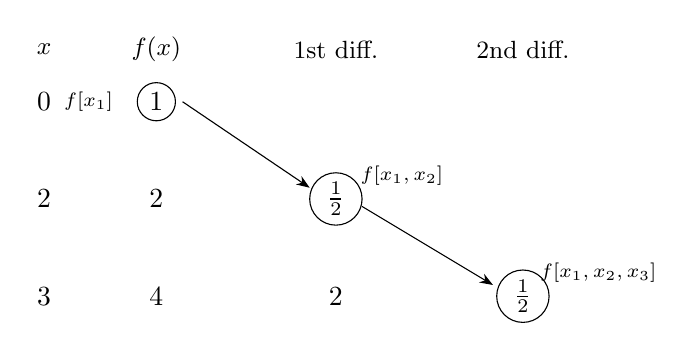
\begin{tikzpicture}[scale=0.95,>=Stealth]
  \node at (0,0.7) {\small $x$}; \node at (1.5,0.7) {\small $f(x)$};
  \node at (3.9,0.7) {\small 1st diff.}; \node at (6.4,0.7) {\small 2nd diff.};
  \node at (0,0) {$0$}; \node[circle,draw,inner sep=2pt] (a) at (1.5,0) {$1$};
  \node at (0,-1.3) {$2$}; \node at (1.5,-1.3) {$2$};
  \node[circle,draw,inner sep=2pt] (b) at (3.9,-1.3) {$\frac12$};
  \node at (0,-2.6) {$3$}; \node at (1.5,-2.6) {$4$};
  \node at (3.9,-2.6) {$2$};
  \node[circle,draw,inner sep=2pt] (c) at (6.4,-2.6) {$\frac12$};
  \draw[->] (1.85,0) -- (3.55,-1.15);
  \draw[->] (4.25,-1.4) -- (6.0,-2.45);
  \node[left] at (1.05,0) {\scriptsize $f[x_1]$};
  \node[above right] at (4.1,-1.25) {\scriptsize $f[x_1,x_2]$};
  \node[above right] at (6.5,-2.55) {\scriptsize $f[x_1,x_2,x_3]$};
\end{tikzpicture}
\end{center}
\[
f[x_1]=1,\qquad
f[x_1,x_2]=\frac{2-1}{2-0}=\frac12,\qquad
f[x_2,x_3]=\frac{4-2}{3-2}=2,\qquad
f[x_1,x_2,x_3]=\frac{2-\frac12}{3-0}=\frac12
\]

\[
\therefore P(x)=1+\frac12(x-0)+\frac12(x-0)(x-2)
\]
\[
=1+\frac{x}{2}+\frac{x(x-2)}{2}
\]

\textbf{Note:} By thm of uniqueness the above $P(x)$ and the one obtained by
Lagrange interpolation must be identical

\subsection*{Proof of Newton's interpolating polynomial:}

Interpolating polynomial of $x_2,x_3,\dots,x_1,x_k$ is
\[
\begin{aligned}
P_1(x)={}&f(x_2)+f[x_2,x_3](x-x_2)+\cdots
+f[x_2,x_3,\dots,x_{k-1},x_k](x-x_2)\cdots(x-x_{k-1})\\
&+f[x_2,\dots,x_{k-1},x_1,x_k](x-x_2)\cdots(x-x_{k-1})(x-x_1)
\end{aligned}
\]
\textbf{(iv)} for $x_2,x_3,\dots,x_{k-1},x_k,x_1$ is
\[
\begin{aligned}
P_2(x)={}&f[x_2]+f[x_2,x_3](x-x_2)+\cdots
+f[x_2,\dots,x_k,x_1](x-x_1)\cdots(x-x_{k-1})(x-x_k)
\end{aligned}
\]
\[
P_1(x)=P_2(x)\qquad\text{(uniqueness)}
\]
\[
\Rightarrow\quad P_1(x_k)=P_2(x_k)
\]
\[
\Rightarrow\quad f[x_2,\dots,x_{k-1},x_1,x_k](x_k-x_2)\cdots(x_k-x_{k-1})
+f[x_2,\dots,x_1,x_k](x_k-x_1)\cdots(x_k-x_{\cdots})
\]

%============================================================
\pagehead{8}

\[
=f[x_2,\dots,x_k](x_k-x_2)\cdots(x_k-x_{k-1})
\]
\[
f[x_2,\dots,x_{k-1},x_k]+f[x_2,\dots,x_{k-1},x_1,x_k](x_k-x_1)
=f[x_2,\dots,x_k]
\]
$\hookrightarrow$ Proof (follows).

\subsection*{Interpolation error}

$P_{n-1}(t)\ \to$ interpolating $n$ data points

Adding $x$ to data points:
\[
P_n(t)=P_{n-1}(t)+f[x_1,\dots,x_n,x](t-x_1)\cdots(t-x_n)
\]
\[
P_n(x)=f(x)=P_{n-1}(x)+f[x_1,\dots,x_n,x](x-x_1)\cdots(x-x_n)
\]
Let
\[
h(t)=f(t)-P_{n-1}(t)-f[x_1,\dots,x_n,x](t-x_1)\cdots(t-x_n)
\]
Now $h(x)=0$; $h(x_1)=\cdots=h(x_n)=0$

b/w each neighbouring pairs of $n+1$ pts, $h'=0$ by Rolle's theorem

We get $n$ such pts where $h'=0$

Now b/w each pair of pts where $h'=0$, $h''=0$

We get $(n-1)$ such pts

\[
\vdots\qquad\text{(successively apply Rolle's theorem)}
\]
$\exists$ one point where $h^{(n)}(t)=0$ \quad (say $t=c$)
\[
h^{(n)}(t)=f^{(n)}(t)-n!\,f[x_1,\dots,x_n,x]
\qquad\because\ [\text{Take }n\text{ derivative of }P_{n-1}(t)=0]
\]
Substitute $c$
\[
\Rightarrow\quad \frac{f^{(n)}(c)}{n!}=f[x_1,\dots,x_n,x]
\qquad\because\ [h^{(n)}(t)=0]
\]

%============================================================
\pagehead{9}

Which leads to
\[
f(x)=P_{n-1}+\frac{f^{(n)}(c)}{n!}(x-x_1)\cdots(x-x_n)
\]

\subsection*{Runge Phenomenon:}

\[
f(x)=\frac{1}{1+12x^2}
\]
$\hookrightarrow$ Matters Lagrange interpolation in center not in boundary

$\hookrightarrow$ error actually increase with no.\ of data pts

However, unequally spaced data points don't experience Runge phenomenon.

\subsection*{Interpolation error}
\[
\text{Interpolation error}=\frac{(x-x_1)\cdots(x-x_n)}{n!}\,f^{(n)}(c)
\]
\[
\omega=(x-x_1)\cdots(x-x_n)\qquad\text{(Neglecting constants)}
\]

\begin{center}
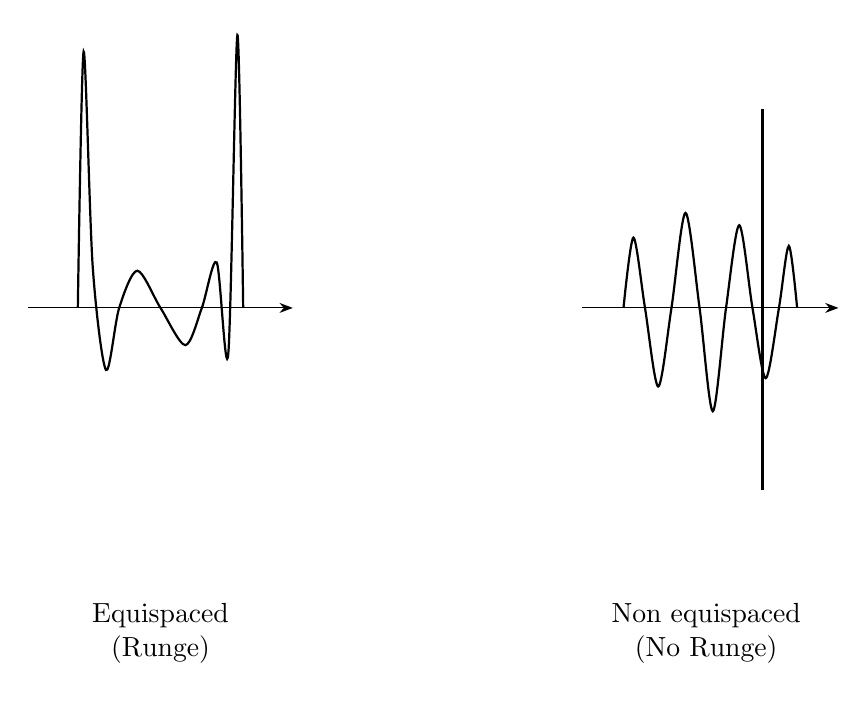
\begin{tikzpicture}[scale=1.05,>=Stealth]
  % left : equispaced
  \begin{scope}[shift={(-4.6,0)}]
    \draw[->] (-1.6,0)--(1.6,0);
    \draw[thick] plot[smooth] coordinates {(-1,0) (-0.93,3.1) (-0.82,0.5)
      (-0.66,-0.75) (-0.5,0) (-0.28,0.45) (0,0) (0.3,-0.45) (0.5,0)
      (0.68,0.55) (0.82,-0.55) (0.93,3.3) (1,0)};
    \node[below] at (0,-3.45) {Equispaced};
    \node[below] at (0,-3.85) {(Runge)};
  \end{scope}
  % right : non-equispaced
  \begin{scope}[shift={(2.0,0)}]
    \draw[->] (-1.5,0)--(1.6,0);
    \draw[thick] plot[smooth] coordinates {(-1,0) (-0.88,0.85) (-0.74,0)
      (-0.58,-0.95) (-0.42,0) (-0.25,1.15) (-0.08,0) (0.08,-1.25)
      (0.24,0) (0.4,1.0) (0.56,0) (0.72,-0.85) (0.88,0) (1,0.75) (1.1,0)};
    \draw[thick] (0.68,-2.2)--(0.68,2.4);
    \node[below] at (0,-3.45) {Non equispaced};
    \node[below] at (0,-3.85) {(No Runge)};
  \end{scope}
\end{tikzpicture}
\end{center}

%============================================================
\pagehead{10}

\subsection*{\underline{Chebyshev's Thm:}}

In the interval $[-1,1]$, $(x-x_1)\cdots(x-x_n)$ is minimized if
\[
(x-x_1)\cdots(x-x_n)=\frac{T_n(x)}{2^{n-1}}
\]
$T_n(x)\to$ Chebyshev polynomial

$n=$ degree of polynomial

$T_n$'s are soln to Sturm--Liouville eqn
\[
\frac{d}{dx}\left[p(x)\frac{dy}{dx}\right]+q(x)y=-\lambda w(x)y
\]
\[
\therefore\ x_i=\cos\left(\frac{2i-1}{2n}\pi\right),\qquad
\text{roots of }T_n(x)
\]
\[
\therefore\ [\text{Roots of Chebyshev polynomial}
=\text{roots of minimal error }[-1,1]]
\]

\textbf{Chebyshev's Thm:} If
$(x-x_1)\cdots(x-x_n)=\dfrac{T_n}{2^{n-1}}$, then
$(x-x_1)\cdots(x-x_n)=\dfrac{1}{2^{n-1}}$

\textbf{Proof:} Assume there is a monic polynomial $P_n(x)$
$\exists\ |P_n(x)|<\dfrac{1}{2^{n-1}}$\\
\hspace*{1.2cm}$\llcorner$ Coeff of leading term $=1$

Since $T_n$ alternates b/w $\pm1$, $n+1$ times,
$P_n-\dfrac{T_n}{2^{n-1}}$ alternates b/w $-$ive and $+$ive
\[
\therefore\ \left[|P_n(x)|<1/2^{n-1}\right]
\]
$\hookrightarrow P_n(x)-\dfrac{T_n(x)}{2^{n-1}}$ \quad crosses zero $n$ times
$\Rightarrow$ It has $n$ roots

$P_n(x)$ is monic and $\dfrac{T_n}{2^{n-1}}$ is also monic
$\Rightarrow P_n-\dfrac{T_n}{2^{n-1}}$ has deg $n-1$ $\longrightarrow$

%============================================================
\pagehead{11}

For general interval:
\[
x_i=\left(\frac{b-a}{2}\right)\cos\left(\frac{2i-1}{2n}\pi\right)
+\frac{b+a}{2}
\]

\subsection*{\# Cubic Splines:}
(a spline is a function defined piecewise)

\begin{center}
\begin{tikzpicture}[scale=0.95,>=Stealth]
  \draw[->] (-0.2,0)--(6.2,0);
  \draw[->] (0.4,-0.2)--(0.4,4.2);
  \fill (1.1,3.2) circle (2pt) node[above] {$P_1$};
  \fill (2.4,3.9) circle (2pt) node[above] {$P_2$};
  \fill (4.2,2.2) circle (2pt) node[right] {$P_3$};
  \fill (2.2,1.4) circle (2pt) node[below left] {$P_4$};
\end{tikzpicture}
\end{center}

$S_1(x)\to$ straight line connecting $P_1-P_2$

$S_2(x)\to$ \phantom{straight line connecting} $P_2-P_3$

\[
\vdots
\]
\[
\therefore\ \text{Interpolating function}=\bigcup S_i
\]
$\hookrightarrow$ Not differentiable at nodes!

$\therefore$ We use cubic splines instead

\begin{center}
\begin{tikzpicture}[scale=0.95,>=Stealth]
  \draw[->] (-0.2,0)--(6.2,0);
  \draw[->] (0.4,-0.2)--(0.4,4.0);
  \draw[thick] plot[smooth] coordinates
    {(0.9,1.5) (1.6,2.5) (2.4,2.9) (3.2,2.4) (3.9,1.6)};
  \fill (0.9,1.5) circle (1.8pt);
  \fill (1.6,2.5) circle (1.8pt);
  \fill (2.4,2.9) circle (1.8pt);
  \fill (3.2,2.4) circle (1.8pt);
  \fill (3.9,1.6) circle (1.8pt);
\end{tikzpicture}
\end{center}

\textbf{Property of cubic splines:}
\begin{enumerate}[label=(\arabic*),leftmargin=2.6em]
\item $S_i(x_i)=y_i$ \quad and \quad $S_i(x_{i+1})=y_{i+1}$
      \quad for $i=1,\dots,n-1$
\item $S'_{i-1}(x_i)=S'_i(x_i)$ \quad $i=2,\dots,n-1$
\item $S''_{i-1}(x_i)=S''_i(x_i)$ \quad $i=2,\dots,n-1$
\end{enumerate}

%============================================================
\pagehead{12}

\[
S_1=y_1+b_1(x-x_1)+c_1(x-x_1)^2+d_1(x-x_1)^3
\quad\text{on }[x_1,x_2]
\]
\[
S_2(x)=y_2+b_2(x-x_2)+c_2(x-x_2)^2+d_2(x-x_2)^3
\quad\text{on }[x_2,x_3]
\]
\[
\vdots
\]
\[
S_{n-1}(x)=y_{n-1}+b_{n-1}(x-x_{n-1})+c_{n-1}(x-x_{n-1})^2
+d_{n-1}(x-x_{n-1})^3
\]

\textbf{Property 1:} $(n-1)$ independent eqn

\textbf{P2:} $(n-2)$ independent eqn

\textbf{P3:} $n-2$ independent eqn

\vspace{-0.2em}
{\color{black!45}\rule{6cm}{0.4pt}}

\[
3n-5\ \text{eqn}
\]
No.\ of unknowns $\Rightarrow 3(n-1)=3n-3$ \quad ($2$ short)

$\therefore$ We set $S''_1(x_1)=0$, $S''_{n-1}(x_n)=0$ to ensure constants are
uniquely determined.

\textbf{Define:}
\[
\delta_i=x_{i+1}-x_i
\]
\[
\Delta_i=y_{i+1}-y_i
\]
\[
b_i=\frac{\Delta_i}{\delta_i}\ ;\qquad
d_i=\frac{c_{i+1}-c_i}{3\delta_i}
\]

\subsection*{Numeric Integration:}

The \emph{degree of precision} of a numerical integration method is the
greatest integer $k$ for which all degree $k$ or less polynomials are
integrated exactly by the method.
\[
\text{The error in trapezoidal}\ \Rightarrow\ -\frac{h^3}{12}f''(c)
\qquad (2\to\text{degree of precision})
\]
\[
\text{''\hspace{1.2cm}Simpson}\ \Rightarrow\ -\frac{h^4}{12}F^{(4)}(c)
\qquad (3\to\text{''\hspace{0.4cm}''\hspace{0.4cm}''})
\]

%============================================================
\pagehead{13}

Simpson uses quadratic but can perfectly integrate a cubic.

\begin{center}
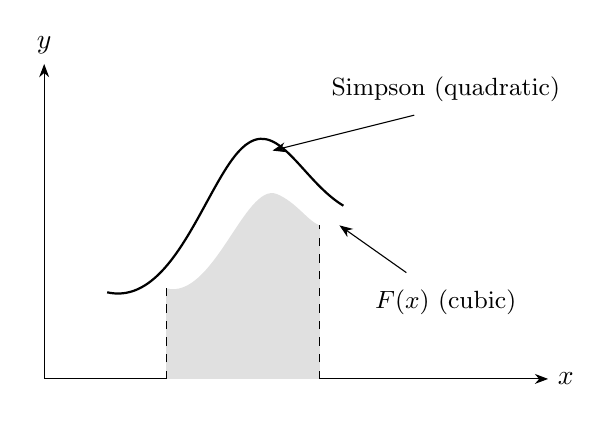
\begin{tikzpicture}[scale=1.0,>=Stealth]
  \draw[->] (0,0)--(6.4,0) node[right] {$x$};
  \draw[->] (0,0)--(0,4.0) node[above] {$y$};
  \draw[thick] (0.8,1.1) .. controls (1.7,0.9) and (2.1,2.7) .. (2.6,3.0)
    .. controls (3.0,3.25) and (3.3,2.5) .. (3.8,2.2);
  \fill[black!12] (1.55,0) -- (1.55,1.15)
    .. controls (2.15,1.0) and (2.55,2.5) .. (2.95,2.35)
    .. controls (3.2,2.25) and (3.35,2.0) .. (3.5,1.95) -- (3.5,0) -- cycle;
  \draw[dashed] (1.55,0)--(1.55,1.15);
  \draw[dashed] (3.5,0)--(3.5,1.95);
  \node[above] at (5.1,3.4) {\small Simpson (quadratic)};
  \draw[->] (4.7,3.35)--(2.9,2.9);
  \node[below] at (5.1,1.25) {\small $F(x)$ (cubic)};
  \draw[->] (4.6,1.35)--(3.75,1.95);
\end{tikzpicture}
\end{center}

\begin{itemize}
\item Midpoint rule
\item Gaussian Quadrature Method
\end{itemize}

\[
\int_{-1}^{1} f(x)\,dx
\]
\[
g(x)=\sum f(x_i)\,l_i(x)
\]
\[
l_i(x)=\prod_{m\neq i}\frac{(x-x_m)}{(x_i-x_m)}
\]
\[
\int_{-1}^{1} f(x)\,dx\approx \int_{-1}^{1} g(x)\,dx
=\sum_{i=1}^{n} c_i f(x_i)
\qquad ;\quad c_i=\int_{-1}^{1} l_i(x)\,dx
\]

\vspace{0.4em}
\begin{center}
$\begin{array}{r|l}
\multicolumn{2}{r}{x^2+x+3}\\
\cline{2-2}
x-3 & x^3-2x^2+0x-4\\
 & -x^3+3x^2\\
\cline{2-2}
 & x^2+0x\\
 & -x^2+3x\\
\cline{2-2}
 & 3x-4\\
 & -3x+9\\
\cline{2-2}
 & 5
\end{array}$
\end{center}
\[
\therefore\quad x^3-2x^2-4=(x-3)(x^2+x+3)+5
\]

%============================================================
\pagehead{14}

\subsection*{System of Eqn}

\[
Ax=b
\]
\[
\left[\begin{array}{ccc|c}
1&2&-1&3\\
2&1&-2&3\\
-3&1&1&-6
\end{array}\right]
\]
\[
\xrightarrow{R_2:\ R_2-2R_1}
\left[\begin{array}{ccc|c}
1&2&-1&3\\
0&-3&0&-3\\
-3&1&1&-6
\end{array}\right]
\]
\[
\xrightarrow{R_3:\ R_3+3R_1}
\left[\begin{array}{ccc|c}
1&2&-1&3\\
0&-3&0&-3\\
0&7&-2&3
\end{array}\right]
\]
\[
\xrightarrow{R_3\to \frac{7R_2}{3}+R_3}
\left[\begin{array}{ccc|c}
1&2&-1&3\\
0&-3&0&-3\\
0&0&-2&-4
\end{array}\right]
\]
\[
\therefore\ x_3=+2
\]
\[
x_2=+1
\]
\[
x_1=3-2+2=3\ \checkmark
\]

Partial Pivoting

\textbf{\underline{LU decomposition:}}

%============================================================
\pagehead{15}

\begin{itemize}
\item Linear ODE
\item $2$nd order Non linear ODEs
\item PDE's
\item Stochastic Systems
\end{itemize}

\[
\frac{dy}{dt}=F(y,t)
\]
$\hookrightarrow$ Discretize
\[
\frac{y(t+\Delta t)-y(t)}{\Delta t}=f(y,t)
\]
\[
\lim_{\Delta t\to 0}\frac{y(t+\Delta t)-y(t)}{\Delta t}=\frac{dy}{dt}
\]
\begin{handbox}
\[
y(t+\Delta t)=y(t)+\Delta t\,F
\]
\end{handbox}

\begin{center}
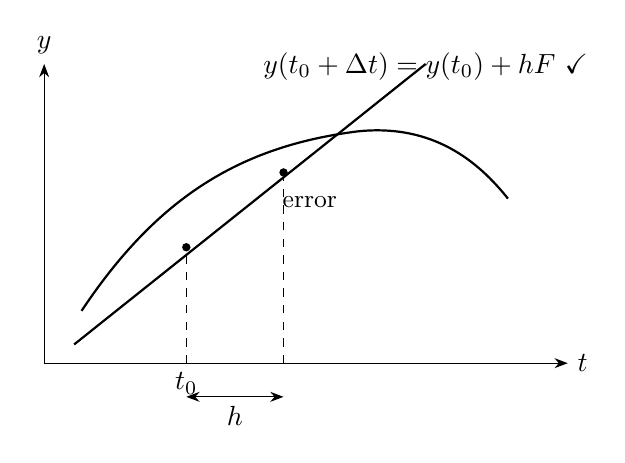
\begin{tikzpicture}[scale=0.95,>=Stealth]
  \draw[->] (0,0)--(7,0) node[right] {$t$};
  \draw[->] (0,0)--(0,4) node[above] {$y$};
  \draw[thick] (0.5,0.7) .. controls (1.5,2.2) and (2.6,2.9) .. (4.2,3.1)
    .. controls (5.2,3.2) and (5.8,2.7) .. (6.2,2.2);
  \draw[thick] (0.4,0.25)--(5.1,4.0);
  \draw[dashed] (1.9,0)--(1.9,1.55);
  \draw[dashed] (3.2,0)--(3.2,2.55);
  \node[below] at (1.9,0) {$t_0$};
  \draw[<->] (1.9,-0.45)--(3.2,-0.45) node[midway,below] {$h$};
  \fill (1.9,1.55) circle (1.6pt);
  \fill (3.2,2.55) circle (1.6pt);
  \node[above right] at (2.8,3.65) {$y(t_0+\Delta t)=y(t_0)+hF$ \checkmark};
  \node at (3.55,2.15) {\small error};
\end{tikzpicture}
\end{center}

$\to$ Simple Euler Method

\[
y(t_0+h)=y_1=y_0+hf_0
\qquad \left(\text{Error}:O(h^2)\right)\to\text{we'll show}
\]
\[
\text{Taylor expansion}\qquad
y(t_0+h)=y(t_0)+h\,y'(t_0)+\frac{h^2}{2!}y''(c)
\]

%============================================================
\pagehead{16}

\[
y_2=y_1+hf_1\qquad\left(\text{Error}\propto O(h^2)\right)
\]
\[
\vdots
\]
\[
y_N=y_{N-1}+hF_{N-1}\qquad\left[\text{Error}:N\,O(h^2)\right]
\]
\[
\text{Local error}: O(h^2)
\]
\[
\text{Global error}: N\,O(h^2)
\qquad
\begin{cases}
N-\text{No.\ of iterations}\\
T-\text{Total time of solving}\\
\Rightarrow T=Nh
\end{cases}
\]
\[
\text{Global error}:\frac{T}{h}O(h^2)
\]
\[
\propto O(h)
\]
\[
\text{Local error}\ll\text{Global error}
\]

\begin{center}
\begin{tikzpicture}[scale=1.0,>=Stealth]
  \draw[->] (-0.3,0)--(7.2,0) node[right] {$t$};
  \draw[->] (0,-0.2)--(0,4.0) node[above] {$x$};
  \draw[thick,domain=0.3:6.8,samples=100] plot (\x,{3.8*exp(-0.65*\x)});
  \draw[dashed] (1.6,0)--(1.6,{3.8*exp(-1.04)});
  \node[below] at (1.6,0) {$a$};
  \node at (3.5,2.4) {$\dfrac{dx}{dt}=-\lambda x$};
  \node at (5.9,3.25) {$\tau=\dfrac{1}{\lambda}$};
  \draw[->] (5.9,2.95)--(5.9,2.55) node[pos=1.1,right] {\small timescale};
\end{tikzpicture}
\end{center}

Choose $\Delta t\ll\tau$ (smaller than timescale of problem)

\# How to set $h/\Delta t$?

\begin{enumerate}[label=(\arabic*)]
\item Convergence
\item Characteristic scales in the system
\end{enumerate}

%============================================================
\pagehead{17}

\subsection*{\underline{Non linear ODE:}}

\[
\frac{dx}{dt}=x(1-x^2)
\]
\begin{center}
\begin{tikzpicture}[scale=1.0,>=Stealth]
  \draw[->] (-2.2,0)--(2.4,0) node[right] {$x$};
  \draw[->] (0,-2.2)--(0,2.4) node[above] {$\dot x$};
  \draw[thick,domain=-1.55:1.55,samples=120] plot (\x,{\x*(1-\x*\x)});
  \node[below] at (-1,-0.22) {$-1$};
  \node[below] at (0.05,-0.22) {$0$};
  \node[below] at (1,-0.22) {$+1$};
\end{tikzpicture}
\end{center}

Steady state $\Rightarrow \dfrac{dx}{dt}=x(1-x^2)=0$
\[
\hookrightarrow x=0,\ \pm1
\]

From graph, given any initial condition $x_0$, we can tell which steady state
the soln will settle to, without knowing closed form soln.

If you start close to a steady state and end up diverging away
$\Rightarrow$ unstable steady state

else $\to$ stable steady state

\subsection*{(Double well potential):}
\[
V=\frac12kx^2-\frac14\lambda x^4
\]
\[
m\ddot x=-\gamma\dot x-\frac{\partial V}{\partial x}
\]
For $\dfrac{m}{\gamma}\ll1$, the 2nd ODE reduces to
$\gamma\dot x=-\dfrac{\partial V}{\partial x}$

Letting $\gamma=1$ we get
\[
\dot x=x(1-x^2)
\]

\subsection*{2 Dimensional System:}
\[
\frac{dx}{dt}=f(x,y)\ ;\qquad \frac{dy}{dt}=g(x,y)
\]
\[
f(x^*,y^*)=0=g(x^*,y^*)\qquad\text{(equilibrium)}
\]

%============================================================
\pagehead{18}

\[
\left.\begin{aligned}
x&=u+x^*\\
y&=v+y^*
\end{aligned}\right\}
\ \to\ \text{perturbations in }x^*\text{ and }y^*
\]
\[
\frac{d}{dt}(u+x^*)=f(u+x^*,v+y^*)
\]
\[
\frac{d}{dt}(v+y^*)=g(u+x^*,v+y^*)
\]
\[
\frac{\partial u}{\partial t}
=f(x^*,y^*)+\underbrace{u\frac{\partial f}{\partial x}(x^*,y^*)
+v\frac{\partial f}{\partial y}(x^*,y^*)}_{0}
\]
\[
\frac{\partial v}{\partial t}
=g(x^*,y^*)+\underbrace{u\frac{\partial g}{\partial x}(x^*,y^*)
+v\frac{\partial g}{\partial y}(x^*,y^*)}_{0}
\]
\[
\Rightarrow\quad \frac{d}{dt}
\begin{bmatrix}u\\v\end{bmatrix}
=
\begin{bmatrix}f_x&f_y\\g_x&g_y\end{bmatrix}
\begin{bmatrix}u\\v\end{bmatrix}
\]
\begin{center}
\small$\hookrightarrow$ Linearization
\end{center}
\[
J=\begin{bmatrix}a&b\\c&d\end{bmatrix}=\text{Jacobian}\ \checkmark
\]
If $\lambda_1,\lambda_2$ are eigenvalues of $J$:
\[
\begin{bmatrix}u\\v\end{bmatrix}=X
=\alpha\,v_1e^{\lambda_1t}+\beta\,v_2e^{\lambda_2t}
\]
\[
\lambda_i\to\text{eigenvalues}\ ;\qquad v_i\to\text{eigenvectors}
\]

%============================================================
\pagehead{19}

\begin{center}
\begin{tikzpicture}[scale=0.95,>=Stealth]
  \draw[->] (-2.6,0)--(2.6,0) node[right] {$v_1$};
  \draw[->] (0,-2.6)--(0,2.6) node[above] {$v_2$};
  \draw[->] (1.9,0)--(0.6,0);
  \draw[->] (-1.9,0)--(-0.6,0);
  \draw[->] (0,1.9)--(0,0.6);
  \draw[->] (0,-1.9)--(0,-0.6);
  \node at (1.95,0.55) {$\lambda_1<0$};
  \node at (0.62,2.12) {$\lambda_2<0$};
  \draw[->] (1.55,0.40) to[bend left=35] (0.42,1.45);
\end{tikzpicture}
\end{center}

\[
|J-\lambda I|=
\begin{vmatrix}
a-\lambda&b\\
c&d-\lambda
\end{vmatrix}=0
\]
\[
\Rightarrow\quad \lambda^2-(a+d)\lambda+ad-bc=0
\]
\[
\Rightarrow\quad \lambda^2-\operatorname{tr}(J)\lambda+\det(J)=0
\]
\[
\Rightarrow\quad \lambda=
\frac{\operatorname{tr}(J)\pm\sqrt{(\operatorname{tr}(J))^2-4\det(J)}}{2}
\]
Let $\operatorname{tr}(J)=\tau$ ; $\det J=\Delta$
\[
\therefore\quad \lambda_{1,2}=\frac{\tau\pm\sqrt{\tau^2-4\Delta}}{2}
\]

\subsection*{CASE I: $\Delta<0$ ; $\tau>0$}
\[
\sqrt{\tau^2-4\Delta}>\tau>0
\]
\[
\hookrightarrow \lambda_1>0\ ;\quad \lambda_2<0
\]
\begin{center}
\begin{tikzpicture}[scale=0.85,>=Stealth]
  \draw[->] (-2.4,0)--(2.4,0) node[right] {$v_1$};
  \draw[->] (0,-2.4)--(0,2.4) node[above] {$v_2$};
  \draw[->] (0.3,0)--(1.9,0);
  \draw[->] (-0.3,0)--(-1.9,0);
  \draw[->] (0,1.7)--(0,0.4);
  \draw[->] (0,-1.7)--(0,-0.4);
\end{tikzpicture}
\end{center}

%============================================================
\pagehead{20}

\subsection*{CASE II: $\Delta>0$}

\textbf{(i)} $\tau^2-4\Delta>0$ ; $\tau>0$
\[
\hookrightarrow \lambda_1,\lambda_2>0
\]
\begin{center}
\begin{tikzpicture}[scale=0.60,>=Stealth]
  \draw[->] (-2.1,0)--(2.1,0) node[right] {$v_1$};
  \draw[->] (0,-2.1)--(0,2.1) node[above] {$v_2$};
  \draw[->] (0.3,0)--(1.7,0); \draw[->] (-0.3,0)--(-1.7,0);
  \draw[->] (0,0.3)--(0,1.7); \draw[->] (0,-0.3)--(0,-1.7);
\end{tikzpicture}
\end{center}

\textbf{(ii)} $\tau^2-4\Delta>0$ ; $\tau<0$
\[
\hookrightarrow \lambda_1,\lambda_2<0
\]
\begin{center}
\begin{tikzpicture}[scale=0.60,>=Stealth]
  \draw[->] (-2.1,0)--(2.1,0) node[right] {$v_1$};
  \draw[->] (0,-2.1)--(0,2.1) node[above] {$v_2$};
  \draw[->] (1.7,0)--(0.3,0); \draw[->] (-1.7,0)--(-0.3,0);
  \draw[->] (0,1.7)--(0,0.3); \draw[->] (0,-1.7)--(0,-0.3);
\end{tikzpicture}
\end{center}

\textbf{(iii)} $\tau^2-4\Delta<0$ ; $\tau>0$
\[
\hookrightarrow \lambda_1,\lambda_2\in\mathbb{C}
\]
\[
\hookrightarrow e^{\tau}e^{i\Box}=\lambda_{\Box}
\]
$\tau>0\Rightarrow$ Anti-Damped

\begin{center}
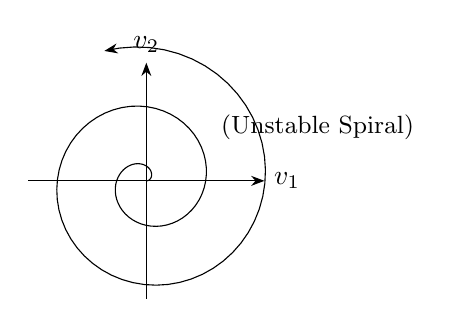
\begin{tikzpicture}[scale=0.75,>=Stealth]
  \draw[->] (-2.0,0)--(2.0,0) node[right] {$v_1$};
  \draw[->] (0,-2.0)--(0,2.0) node[above] {$v_2$};
  \draw[->,domain=0:4.6*pi,samples=130] plot
    ({0.16*\x*cos(\x r)},{0.16*\x*sin(\x r)});
  \node at (2.9,0.9) {\small (Unstable Spiral)};
\end{tikzpicture}
\end{center}

\textbf{(iv)} $\tau^2-4\Delta<0$ ; $\tau<0$ \quad (Damped Spiral)

\begin{center}
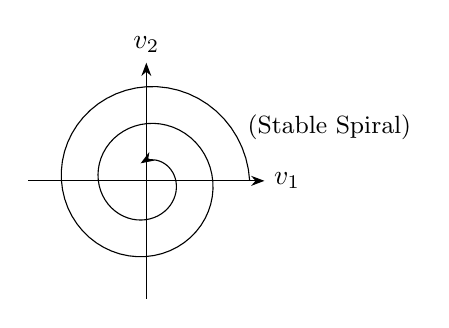
\begin{tikzpicture}[scale=0.75,>=Stealth]
  \draw[->] (-2.0,0)--(2.0,0) node[right] {$v_1$};
  \draw[->] (0,-2.0)--(0,2.0) node[above] {$v_2$};
  \draw[->,domain=0:4.6*pi,samples=130] plot
    ({1.75*(1-\x/(5.6*pi))*cos(\x r)},{1.75*(1-\x/(5.6*pi))*sin(\x r)});
  \node at (3.1,0.9) {\small (Stable Spiral)};
\end{tikzpicture}
\end{center}

%============================================================
\pagehead{21}

\textbf{(v)} $\tau^2-4\Delta<0$ ; $\tau=0$

\begin{center}
\begin{tikzpicture}[scale=0.95,>=Stealth]
  \draw[->] (-2.3,0)--(2.3,0) node[right] {$v_1$};
  \draw[->] (0,-2.3)--(0,2.3) node[above] {$v_2$};
  \draw[thick] (0,0) ellipse (1.35 and 1.0);
  \draw[->] (1.35,0.1) arc (10:70:1.35 and 1.0);
  \draw[->>] (-1.35,-0.1) arc (190:250:1.35 and 1.0);
  \node at (3.2,1.1) {\small (Centre)};
\end{tikzpicture}
\end{center}

\textbf{(vi)}
\[
\dot x=x(3-x-2y)
\]
\[
\dot y=y(2-x-y)
\]
\[
0=x(3-x-2y)
\]
\[
0=y(2-x-y)
\]
\[
3-x-2y=0
\]
\begin{handbox}
\[
\begin{array}{cc}
\boxed{x=y=0} & \boxed{y=0,\ x=3}\\[8pt]
\boxed{x=0,\ y=2} &\\[4pt]
\boxed{x=y=1} &
\end{array}
\]
\end{handbox}

\subsection*{\underline{Partial differential eqn}}

\[
\frac{\partial P}{\partial t}=F(P,t)
\]
\[
\frac{\partial P}{\partial t}=D\,\frac{\partial^2P}{\partial x^2}
\]

\begin{center}
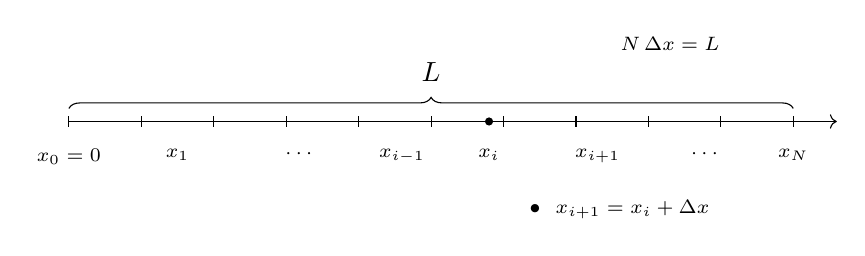
\begin{tikzpicture}[scale=0.92]
  \draw[->] (0,0)--(10.6,0);
  \foreach \x in {0,1,...,10} \draw (\x,0.07)--(\x,-0.07);
  \node[below] at (0,-0.25) {\scriptsize $x_0=0$};
  \node[below] at (1.5,-0.25) {\scriptsize $x_1$};
  \node[below] at (3.2,-0.25) {\scriptsize $\cdots$};
  \node[below] at (4.6,-0.25) {\scriptsize $x_{i-1}$};
  \node[below] at (5.8,-0.25) {\scriptsize $x_i$};
  \node[below] at (7.3,-0.25) {\scriptsize $x_{i+1}$};
  \node[below] at (8.8,-0.25) {\scriptsize $\cdots$};
  \node[below] at (10.0,-0.25) {\scriptsize $x_N$};
  \draw[decorate,decoration={brace,amplitude=4pt}] (0,0.18)--(10.0,0.18);
  \node[above] at (5.0,0.42) {$L$};
  \node[above] at (8.3,0.85) {\scriptsize $N\,\Delta x=L$};
  \fill (5.8,0) circle (1.6pt);
  \node[below] at (7.6,-0.95) {\scriptsize $\bullet\ \ x_{i+1}=x_i+\Delta x$};
\end{tikzpicture}
\end{center}

\[
\frac{\partial F}{\partial x}=\frac{F(x_{i+1})-F(x_i)}{\Delta x}
=\frac{F(x+\Delta x)-F(x)}{\Delta x}
\]
Also
\[
\frac{\partial F}{\partial x}=\frac{F(x_i)-F(x_{i-1})}{\Delta x}
=\frac{F(x_{i+1})-F(x_{i-1})}{2\Delta x}
\]

%============================================================
\pagehead{22}

Coming back to diffusion eqn:

Discretize 2nd order derivatives
\[
\frac{\partial^2F}{\partial x^2}
=\frac{\partial}{\partial x}\left(\frac{F(x+\Delta x)-F(x)}{\Delta x}\right)
\qquad\text{(Forward scheme)}
\]
\[
=\frac{F(x+\Delta x)-F(x)-(F(x)-F(x-\Delta x))}{(\Delta x)^2}
\qquad\text{(Backward scheme)}
\]
\[
=\frac{F(x+\Delta x)-2F(x)+F(x-\Delta x)}{(\Delta x)^2}
\]
\[
\Rightarrow\quad
\frac{P(x,t_n+\Delta t)-P(x,t_n)}{\Delta t}
=D\,\frac{\partial^2P}{\partial x^2}
\]
\[
P(x,t_n+\Delta t)=P(x,t_n)+D\Delta t\,\frac{\partial^2P}{\partial x^2}
\]
\[
=P(x_i,t_n)+\frac{D\Delta t}{\Delta x^2}
\left[P(x_{i+1},t_n)+P(x_{i-1},t_n)-2P(x_i,t_n)\right]
\]
\begin{handbox}
\[
P_i^{\,n+1}=P_i^{\,n}
+\frac{D\Delta t}{\Delta x^2}
\left(P_{i+1}^{\,n}+P_{i-1}^{\,n}-2P_i^{\,n}\right)
\]
\end{handbox}
\begin{center}
\small$\hookrightarrow$ Discretization of Diffusion
\end{center}
\[
P_i^{\,n}=T^nX_i
\]
\[
=T^n\sum_{j=1}^{N}e^{ik_jx_i}\hat X_j
\qquad ;\quad
f(x)=\int e^{ikx}\hat f(k)\,dk
\]
\begin{handbox}
\centering
$\text{Sol}^n=\text{Temporal}\ \times\ \text{Spatial part}$
\end{handbox}

%============================================================
\pagehead{23}

\[
\downarrow
\]
\begin{center}
\textbf{In Fourier transform}
\end{center}

Substitute this in discretization:
\begin{multline*}
T^{n+1}\left(\sum_{j=1}^{N}e^{ik_jx_i}\hat X_j\right)
=T^n\left(\sum_{j=1}^{N}e^{ik_jx_i}\hat X_j\right)
+\frac{D\Delta t}{\Delta x^2}\Biggl[T^n\left(\sum_{j=1}^{N}
e^{ik_j(x_i+\Delta x)}\hat X_j\right)\\
+T^n\sum_{j=1}^{N}e^{ik_j(x_i-\Delta x)}\hat X_j
-2T^n\sum_{j=1}^{N}e^{ik_jx_i}\hat X_j\Biggr]
\end{multline*}

For $j$th component,
\begin{multline*}
T^{n+1}e^{ik_jx_i}\hat X_j
=T^ne^{ik_jx_i}\hat X_j
+C\hat X_jT^n\Bigl[e^{ik_j(x_i+\Delta x)}
+e^{ik_j(x_i-\Delta x)}-2e^{ik_jx_i}\Bigr]
\end{multline*}
\begin{handbox}
\[
C=-\frac{D\Delta t}{\Delta x^2}
\]
\end{handbox}
\[
\Rightarrow\quad T^{n+1}\hat X_j
=T^n\hat X_j+C\hat X_jT^n
\left[e^{ik_j\Delta x}+e^{-ik_j\Delta x}-2\right]
\]
\begin{handbox}
\[
T^{n+1}=T^n\left[1+C\left(2\cos(k_j\Delta x)-2\right)\right]
\]
\end{handbox}
\[
\hookrightarrow T^{n+1}=T^n\left[1-4C\sin^2\left(\frac{k_j\Delta x}{2}\right)\right]
\]
We need $T^{n+1}\le T^n$
\[
\left|1-4C\sin^2\left(\frac{k_j\Delta x}{2}\right)\right|\le1
\]
\[
\hookrightarrow -(1-4C)\le1
\qquad\Longrightarrow\qquad
\boxed{C\le\frac12}
\]
\begin{handbox}
\[
\frac{D\Delta t}{\Delta x^2}\le\frac12
\]
\end{handbox}
\[
\longrightarrow\quad\text{Neumann stability condition}
\]

%============================================================
\pagehead{24}

\subsection*{\underline{Wave Eqn:}}
\[
\frac{\partial^2\psi}{\partial t^2}=c^2\frac{\partial^2\psi}{\partial x^2}
\]
\[
\downarrow
\]
\[
\frac{\partial\psi}{\partial t}=c\,\frac{\partial\psi}{\partial x}
\]
\[
\psi=F(x-ct)=e^{-(x-ct)^2}
\qquad\text{(Rightward travelling wave)}
\]
\[
\frac{\partial\psi}{\partial t}
=e^{-(x-ct)^2}(+2)(x-ct)\,c
\]
\[
\frac{\partial\psi}{\partial x}
=e^{-(x-ct)^2}(-2)(x-ct)
\]
\[
\hookrightarrow\quad
\frac{\partial\psi}{\partial t}=-c\,\frac{\partial\psi}{\partial x}
\qquad\checkmark\quad(\text{works for gaussian!})
\]

2nd eqn is not gradient with $x-ct$ : thus backward wave is not a soln to
2nd eqn

Mechanism of wave propagation in 2nd order $\to$ Advection

To describe Advection + Diffusion:
\begin{handbox}
\[
\frac{\partial P}{\partial t}
=D\,\frac{\partial^2P}{\partial x^2}-c\,\frac{\partial P}{\partial x}
\]
\end{handbox}

%============================================================
\pagehead{25}

\subsection*{\underline{Coming Back to Advection:}}

\[
\frac{\psi_i^{\,n+1}-\psi_i^{\,n}}{\Delta t}
=-c\left(\frac{\psi_i^{\,n}-\psi_{i-1}^{\,n}}{\Delta x}\right)
\]
\[
\Rightarrow\quad \psi_i^{\,n+1}
=\psi_i^{\,n}-\frac{c\Delta t}{\Delta x}
\left(\psi_i^{\,n}-\psi_{i-1}^{\,n}\right)
\]

\subsection*{Stability condition.}

\[
\psi_i^{\,n}=T^nX_i\ ;\qquad
X_i=\sum_j e^{ik_jx_i}\hat X_j
\]
Substituting
\begin{multline*}
T^{n+1}\sum_i e^{ik_jx_i}\hat X_j
=T^n\sum_j e^{ik_jx_i}\hat X_j
-\frac{c\Delta t}{\Delta x}\Biggl[T^n\sum_j e^{ik_jx_i}\hat X_j\\
-T^n\sum_j e^{ik_j(x_i-\Delta x)}\hat X_j\Biggr]
\end{multline*}

For $j$th mode:
\begin{multline*}
T^{n+1}e^{ik_jx_i}\hat X_j
=T^ne^{ik_jx_i}\hat X_j
-\frac{c\Delta t}{\Delta x}
\left[T^ne^{ik_jx_i}\hat X_j
-T^ne^{ik_j(x_i-\Delta x)}\hat X_j\right]
\end{multline*}
\[
T^{n+1}=T^n-\frac{c\Delta t}{\Delta x}
\left[T^n-e^{-ik_j\Delta x}T^n\right]
\]
\begin{handbox}
\[
T^{n+1}=T^n\left[1+e^{-ik_j\Delta x}\frac{c\Delta t}{\Delta x}
-\frac{c\Delta t}{\Delta x}\right]
\]
\end{handbox}
Let
\[
K=\frac{c\Delta t}{\Delta x}
\]

%============================================================
\pagehead{26}

\[
T^{n+1}=T^n\left[1-K\left(1-e^{-ik_j\Delta x}\right)\right]
\]
We impose the condition that
\[
\left|1-K\underbrace{\left(1-e^{-ik_j\Delta x}\right)}_{\text{max val }=2}\right|\le1
\]
\[
\longrightarrow\quad -(2K+1)\le1
\]
\[
\Rightarrow\quad 2K-1\ge1
\]
\[
\Rightarrow\quad \boxed{K\le1}
\]
\begin{handbox}
\[
\frac{C\Delta t}{\Delta x}\le1
\quad\to\quad\text{stability condition for 1st order wave eqn}
\]
\end{handbox}
\begin{handbox}
\[
c\le\frac{\Delta x}{\Delta t}
\]
\end{handbox}
\[
\longrightarrow\quad \text{rate of updating}>\text{velocity}
\]

\subsection*{2nd order Wave eqn:}
\[
\frac{\psi_i^{\,n+1}+\psi_i^{\,n-1}-2\psi_i^{\,n}}{(\Delta t)^2}
=c^2\left(
\frac{\psi_{i+1}^{\,n}+\psi_{i-1}^{\,n}-2\psi_i^{\,n}}{(\Delta x)^2}
\right)
\]
\[
\psi_i^{\,n+1}
=\frac{c^2\Delta t^2}{\Delta x^2}
\left(\psi_{i+1}^{\,n}+\psi_{i-1}^{\,n}\right)
+2\left(1-\frac{c^2\Delta t^2}{\Delta x^2}\right)\psi_i^{\,n}
-\psi_i^{\,n-1}
\]

%============================================================
\pagehead{27}

\[
\psi_i^{\,1}=K^2\left(\psi_{i+1}^{\,0}+\psi_{i-1}^{\,0}\right)
+2\left(1-K^2\right)\psi_i^{\,0}-\psi_i^{-1}
\]
Initial condition (known)
\[
\left.\frac{\partial\psi}{\partial t}\right|_{t=0}
=\frac{\psi_i^{\,1}-\psi_i^{-1}}{2\Delta t}
\]
\[
\Rightarrow\quad -2\Delta t\left(\left.\frac{\partial\psi}{\partial t}
\right|_{t=0}\right)+\psi_i^{\,1}=\psi_i^{-1}
\]
\begin{handbox}
\[
\therefore\quad \psi_i^{-1}
=\psi_i^{\,1}-2\Delta t\left(\left.\frac{\partial\psi}{\partial t}
\right|_{t=0}\right)
\]
\end{handbox}
\begin{handbox}
\[
\psi_i^{\,1}
=\frac{K^2}{2}\left(\psi_{i+1}^{\,0}+\psi_{i-1}^{\,0}\right)
+\left(1-K^2\right)\psi_i^{\,0}
+\Delta t\left.\frac{\partial\psi}{\partial t}\right|_{t=0}
\]
\end{handbox}
\[
K=\frac{\Delta x}{\Delta t}
\quad\longrightarrow\quad \text{exact soln (For 2nd order)}
\]

\begin{notebox}[Inserted photograph in the original]
The lower part of page 27 is a photograph of a separate sheet containing the
following Taylor expansions:
\[
\psi(x+\Delta x)=\psi(x)+\Delta x\frac{\partial\psi}{\partial x}
+\frac{\Delta x^2}{2!}\frac{\partial^2\psi}{\partial x^2}+\cdots
\]
\[
\psi(x-\Delta x)=\psi(x)-\Delta x\frac{\partial\psi}{\partial x}
+\frac{\Delta x^2}{2!}\frac{\partial^2\psi}{\partial x^2}+\cdots
\]
\[
\frac{\partial^2\psi}{\partial x^2}
=\frac{\psi(x+\Delta x)+\psi(x-\Delta x)-2\psi}{\Delta x^2}
-\frac{2\Delta x^2}{4!}\frac{\partial^4\psi}{\partial x^4}
-\frac{2\Delta x^4}{6!}\frac{\partial^6\psi}{\partial x^6}+\cdots
\]
Similarly,
\[
\frac{\partial^2\psi}{\partial t^2}
=\frac{\psi(t+\Delta t)+\psi(t-\Delta t)-2\psi}{\Delta t^2}
-\frac{2\Delta t^2}{4!}\frac{\partial^4\psi}{\partial t^4}
-\frac{2\Delta t^4}{6!}\frac{\partial^6\psi}{\partial t^6}+\cdots
\]
\end{notebox}

%============================================================
\pagehead{28}

\subsection*{Derivation of Fokker Planck eqn}

\[
\frac{\partial P}{\partial t}=-\nabla\cdot\vec J
\qquad\text{(continuity eqn)}
\]
\[
\vec J_{\text{diffusion}}+\vec J_{\text{drift}}=\vec J
\]
\[
\vec J_{\text{diffusion}}=-D\frac{\partial P}{\partial x}
\]
\[
\vec J_{\text{drift}}=-P\frac{\partial\Phi}{\partial x}
\]
\begin{handbox}
\[
\frac{\partial P}{\partial t}
=\frac{\partial}{\partial x}
\left[D\frac{\partial P}{\partial x}+P\frac{\partial\Phi}{\partial x}\right]
\]
\end{handbox}

%============================================================
\pagehead{29}

\begin{center}
\emph{(This page is blank in the original.)}
\end{center}

\end{document}
